\subsubsection{Modèle des bandes : un outil pour comprendre l'optimisation des propriétés rédox}
%Chem. Mater. 2010, 22, 587–603 587, DOI:10.1021/cm901452z

\setcounter{equation}{0}
\setcounter{Q}{0}

Dans cette étude, les chercheurs ont acquis les profils de décharge de $4$ matériaux communément utilisés dans les batteries Li-ion en fonction de la st{\oe}chiométrie du lithium \ce{Li}.

\begin{center}
\begin{minipage}[]{0.6\textwidth}

\includegraphics[height=5cm]{Ex17/Fig01}
\end{minipage}\begin{minipage}[]{0.3\textwidth}
\captionof{figure}{Profil de potentiel en décharge, par rapport au couple \ce{Li+}/\ce{Li^0} , des cathodes \ce{Li_x C_6} , \ce{Li_x Ti S_2} and \ce{Li_x [Ti_2] S_4} , \ce{Li_x Co O_2} , and \ce{Li_x Co PO_4}}
\label{fig:17-01}
\end{minipage}
\end{center}
Pour la suite de l'exercice, on assimilera le potentiel mesuré au potentiel de circuit ouvert, et on supposera que le pôle $\ominus$ est la pseudo-référence $\ce{Li^+} | \ce{Li}$.


\Q Au vu des performances du graphite, identifier le rôle de ce type de matériau dans les batteries lithium-ion.
\solution{On constate que le graphite a un $V_{OC}$ compris entre 0.2 et \SI{1}{\volt} en fonction de son degré de lithiation. On en déduit que l'écart entre le potentiel de Fermi d'un pôle $\ominus$ en lithium et un pôle $\oplus$ en graphite est comprise entre 0.2 et \SI{1}{\electronvolt}. \\
Dans les technologies lithium-ion, l'électrode $\ominus$ en lithium métal est remplacée par des électrodes en graphite $\ominus$ du fait des performances similaires.
}

\Q \'{E}crire les demi-équations rédox rendant compte de la lithiation des quatre matériaux étudiés. Dans un modèle purement ionique, en déduire la variation de degré d'oxydation du métal, quand il existe. Le métal subit-il une oxydation ou une réduction lors de la lithiation ?
\solution{Demi-équations rédox et variation du nombre d'oxydation :
\begin{align*}
\ce{x Li^+ + x e^- + C_6 &= Li_xC6} \\
\ce{x Li^+ + x e^- + TiS2 &= Li_xTiS2} \quad no( \ce{Ti}) = +IV \to no( \ce{Ti}) = +III \\
\ce{x Li^+ + x e^- + CoO2 &= Li_xCoO2} \quad no( \ce{Co}) = +IV \to no( \ce{Co}) = +III \\
\ce{x Li^+ + x e^- + CoPO4 &= Li_xCoPO4} \quad no( \ce{Co}) = +III \to no( \ce{Co}) = +II
\end{align*}
Pour les trois métaux, lors de la lithiation, la variation $\Delta no$ de degré d'oxydation faut $-I$. Par rédox interne, le métal subit une réduction.}

\Q \label{Q:17-03} Estimer le potentiel moyen de circuit-ouvert de chacun des matériaux.
\solution{On fait une estimation rudimentaire du potentiel moyen de chacune des électrodes :
\begin{center}
\begin{tabular}{cc}
\ce{Li_xC6} & $\bar{V}_{oc} \approx 0.2 ~ \si{\volt\per{Li^+/Li}}$ \\
\ce{Li_xTiS2} & $\bar{V}_{oc} \approx 2.3 ~ \si{\volt\per{Li^+/Li}}$ \\
\ce{Li_xCoO2} & $\bar{V}_{oc} \approx 4.0 ~ \si{\volt\per{Li^+/Li}}$ \\
\ce{Li_xCoPO4} & $\bar{V}_{oc} \approx 4.7 ~ \si{\volt\per{Li^+/Li}}$
\end{tabular}
\end{center}}

\Q \label{Q:17-04} En quoi la mesure de la tension à circuit-ouverte (OCV), notée $V_{oc}$, permet-elle de sonder la position du niveau de Fermi au pôle $\oplus$. Expliciter la relation existant entre ces différents termes.
% e Voc = \Delta E_F
\solution{La tension à circuit ouverte, liée à la force électromotrice de la cellule électrochimique, est liée au potentiel chimique par la relation : 
\begin{align*}
- F[\si{\coulomb\per\mole}] V_{OC}[\si{\volt}] = \mu_{e^-}^{\oplus} [\si{\joule\per\mole}] - \mu_{e^-}^{\ominus} [\si{\joule\per\mole}]
\end{align*}
résultant de l'interprétation du transfert d'un électron entre deux phases $\oplus$|$\ominus$.
\`{A} \SI{0}{\kelvin}, on sait que le potentiel chimique est proportionnel au niveau de Fermi, à un facteur de conversion d'unité près : 
\begin{align*}
\SI{1}{\joule\per\mole} &= \SI{1}{\coulomb\volt\per\mole} \\
&= \frac{1}{N_A e} ~ \si{\electronvolt} \\
&= \frac{1}{F} ~ \si{\electronvolt}
\end{align*}
On trouve alors la relation simplifiée suivante permettant de facilement interpréter les courbes de charge/décharge en terme d'énergie : 
\begin{align*}
-V_{OC} = \epsilon_F^\oplus - \epsilon_F^\ominus
\end{align*}
avec $\epsilon_F^k$ exprimés en \si{\electronvolt} et la tension $V_{OC}$ exprimée en \si{\volt}.
}

\paragraph*{Relation entre la tension à courant nul et le diagramme de bande}

Les profils de potentiel à circuit-ouvert peuvent souvent être interprétés à l'aide de la structure électronique des matériaux. On se propose de faire cette interprétation. Pour cela, une représentation schématique de la structure de bande des 4 matériaux est proposée.

\begin{figure}[H]
\begin{center}
\begin{tabular}{cc}
\subfloat[\label{fig:17-02a}]{
\includegraphics[height=5cm]{Ex17/Fig02a}} & \subfloat[\label{fig:17-02b}]{
\includegraphics[height=5cm]{Ex17/Fig02b}} \\
\subfloat[\label{fig:17-02c}]{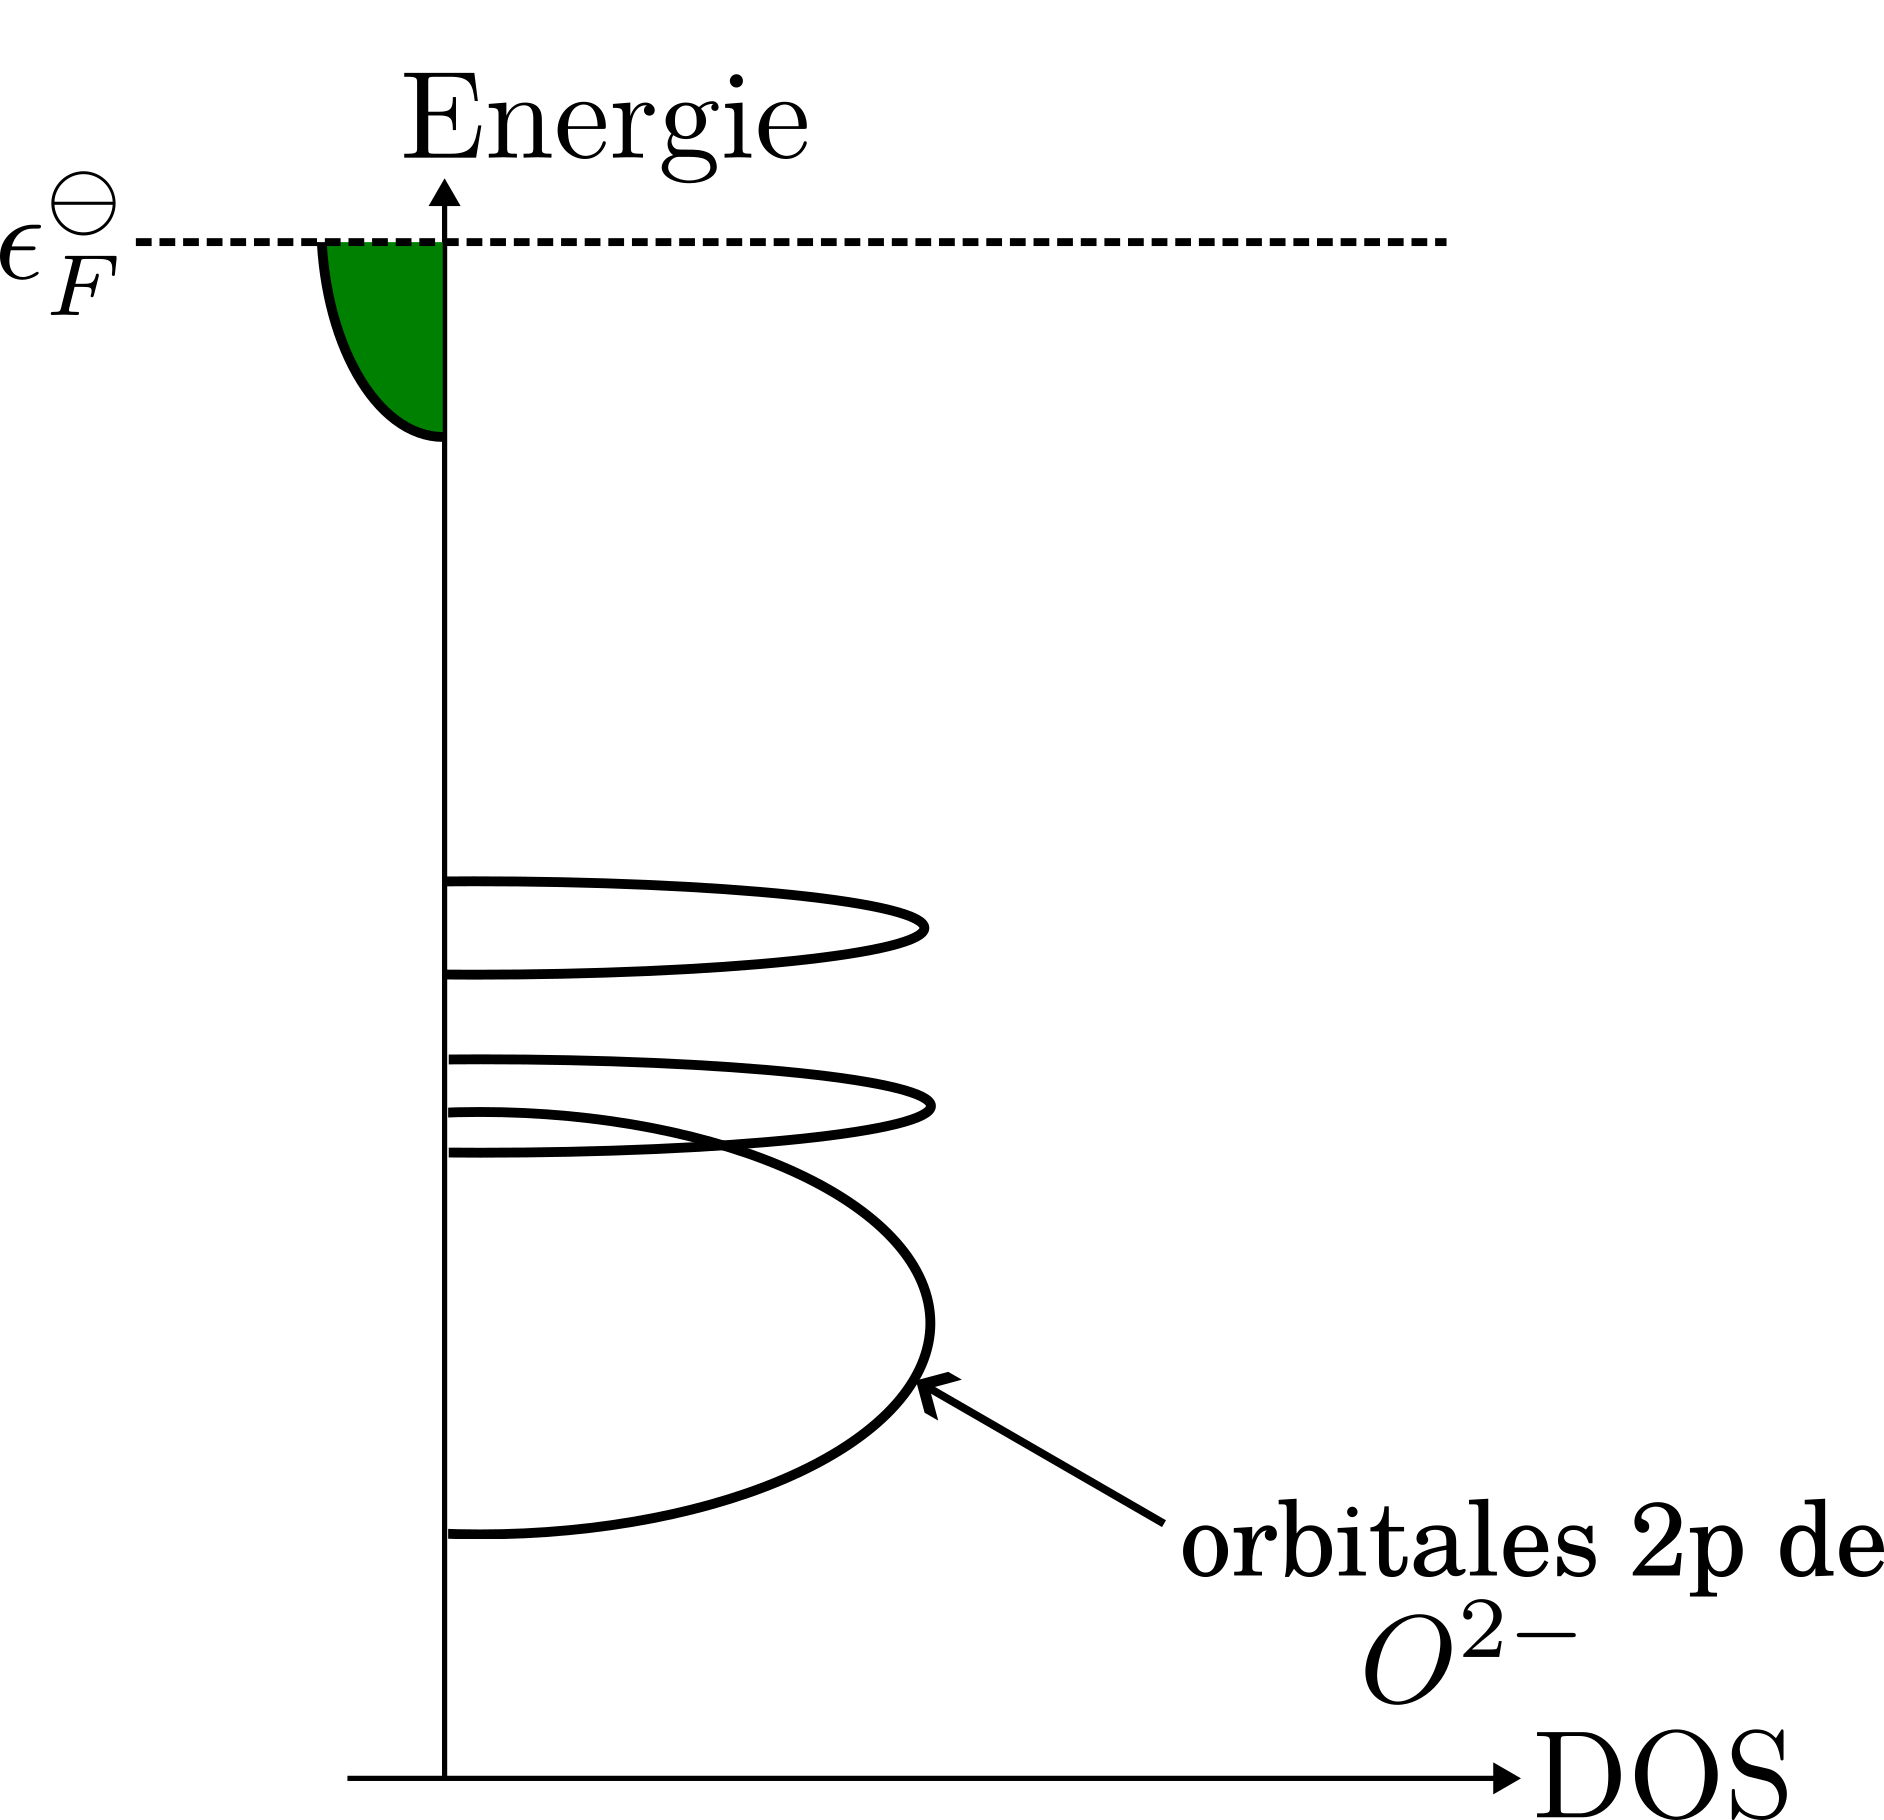
\includegraphics[height=5cm]{Ex17/Fig02c}} & \subfloat[\label{fig:17-02d}]{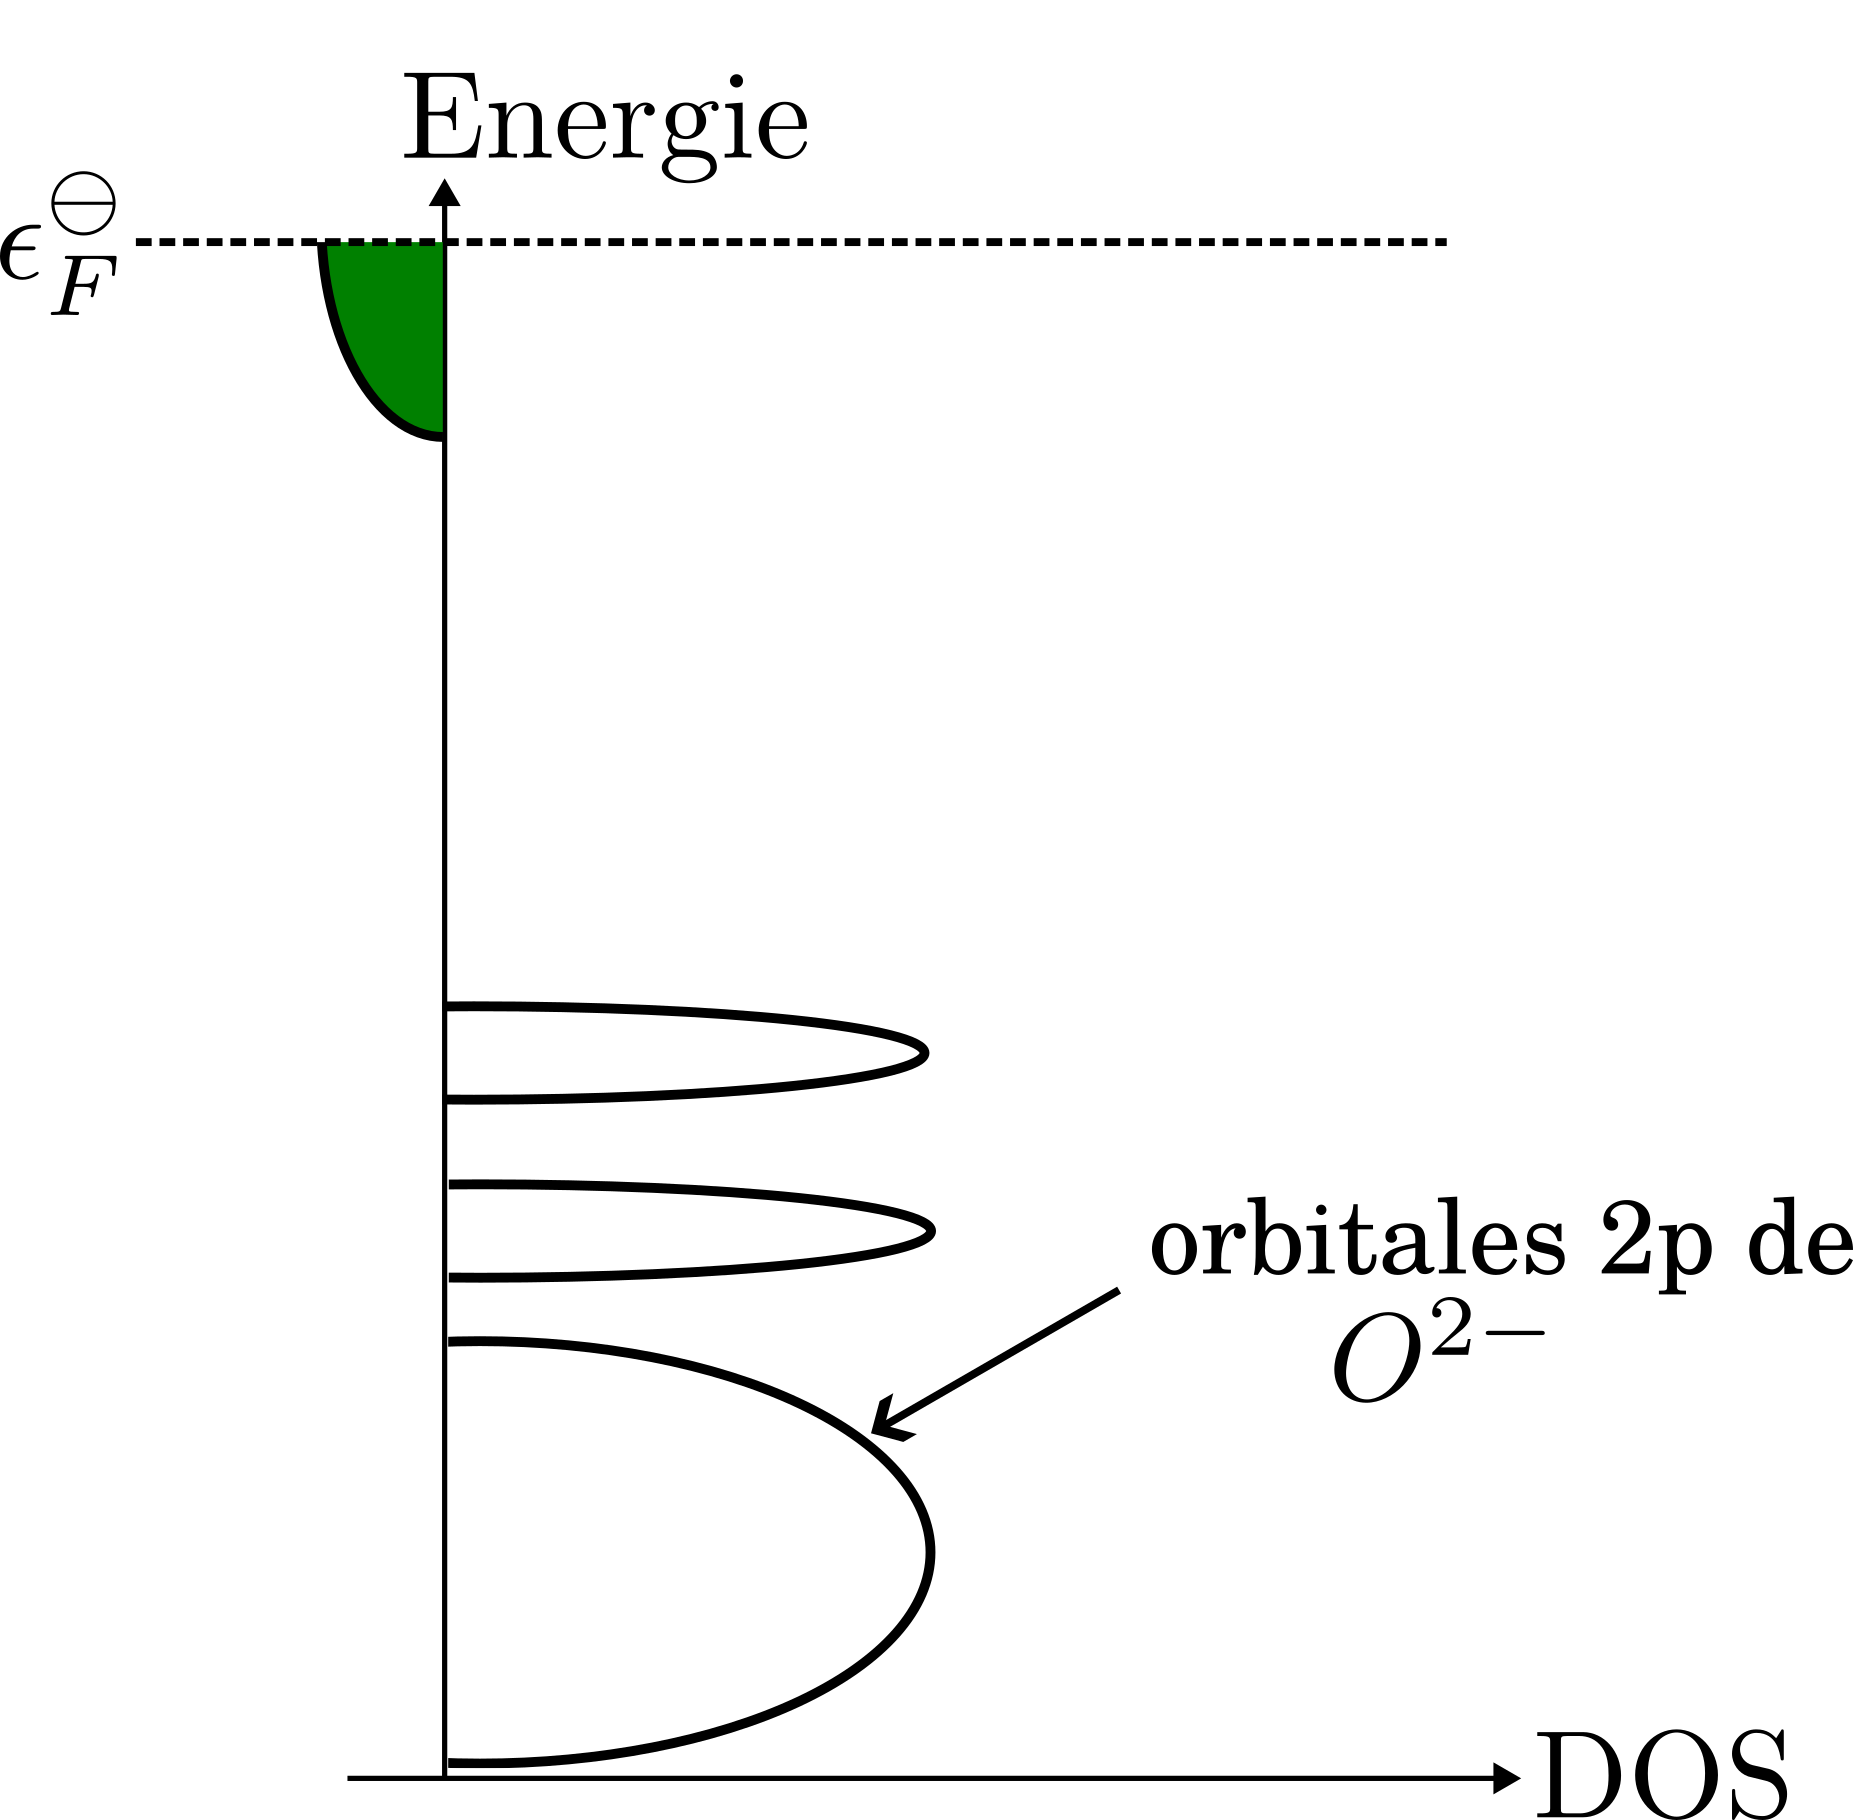
\includegraphics[height=5cm]{Ex17/Fig02d}}
\end{tabular}
\end{center}
\caption{Représentation des orbitales impliquées dans les processus rédox dans \ref{fig:17-02a} \ce{Li_xC6}, \ref{fig:17-02b} \ce{Li_xTiS2}, \ref{fig:17-02c} \ce{Li_xCoO2} et \ref{fig:17-02d} \ce{Li_xCoPO4}}
\end{figure}

On précise que pour les matériaux présentant un métal de transition, le métal est lié aux anions par des octaèdres.

\Q Les bandes étroites d'énergie sont associées aux orbitales du métal. Quelles sont ces orbitales ? Pourquoi les bandes sont étroites ?
\solution{Les bandes étroites correspondent à des orbitales $d$ du métal, lesquelles interagissent faiblement entre elles et avec les autres orbitales du milieu (modèle de liaison fortement ionique). Par conséquent, on a deux bandes étroites : $e_g$ ($d_{x^2-y^2}$, $d_{z^2}$) et $t_{2g}$ ($d_{xy}$, $d_{yz}$, $d_{xz}$).}

\Q Justifier en quoi l'existence d'une bande d'énergie étroite est une garantie de stabilité des cathodes.
\solution{Dans une liaison fortement ionique, le métal est le principal élément à se réduire lors de la lithiation. Lors de la réduction, on peuple des orbitales $d$ anti-liantes du métal. Si la bande peuplée est étroite, on s'attend à avoir une déstabilisation électronique relativement faible (=niveaux anti-liants très proches des niveaux liants).}

\Q Dans la Fig. \ref{fig:17-02a}, les orbitales $2s$ du lithium solvaté dans une matrice de graphite sont représentées. Indiquer le niveau de Fermi lorsque \ce{LiC6} est lithiée.
\solution{
La structure électronique de l'atome de lithium dans \ce{LiC6} est : 
\begin{align*}
[\ce{Li}] = ~_2[\ce{He}] 2s^1
\end{align*}
On s'attend à avoir une orbitale $2s$ demi-pleine et, d'après les Q. \ref{Q:17-03} et \ref{Q:17-04}, la différence d'énergie entre les niveaux de Fermi est de \SI{0.2}{\electronvolt}. On colorie la moitié de l'aire sous la densité d'état de l'orbitale $2s$ : 
\begin{center}
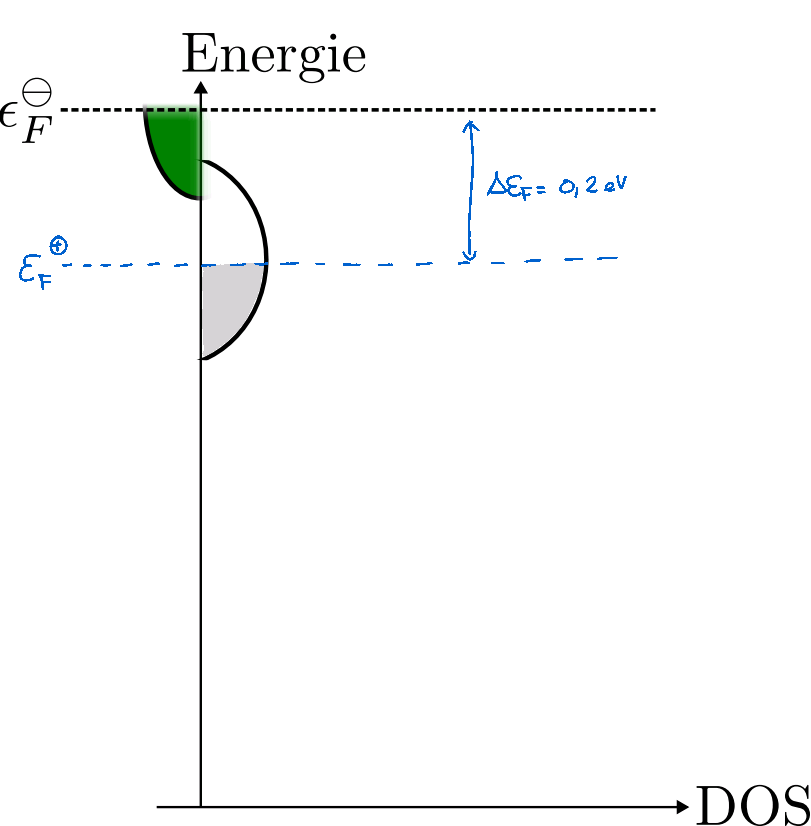
\includegraphics[height=5cm]{Ex17/Corr01a}
\end{center}}

\Q Pour chacun des oxydes métalliques, calculer le nombre d'électrons de valence.
\solution{D'après les règles de l'Aufbau, 
\begin{align*}
[\ce{Ti}] &: ~ _{18}[Ar] 4s^2 3d^2 \\
&\implies [\ce{Ti^{3+}}] : ~ _{18}[Ar] 3d^1 4s^0 \implies \text{1 électron de valence} \\
&\implies [\ce{Ti^{4+}}] : ~ _{18}[Ar] 3d^0 4s^0 \implies \text{0 électron de valence} \\
[\ce{Co}] &: ~ _{18}[Ar] 4s^2 3d^7 \\
&\implies [\ce{Co^{2+}}] : ~_{18}[Ar] 3d^7 4s^0 \implies \text{7 électrons de valence}\\
&\implies [\ce{Co^{3+}}] : ~_{18}[Ar] 3d^6 4s^0 \implies \text{6 électrons de valence}\\
&\implies [\ce{Co^{4+}}] : ~_{18}[Ar] 3d^5 4s^0 \implies \text{5 électrons de valence}
\end{align*}}

\Q Dans une approximation de liaison ionique, proposer un remplissage électronique pour chacun des matériaux lithiés.
\solution{Sachant que les configurations électornique des anions valent $p^6$, et que les configurations des métaux valent : \ce{LiTiS2} - $d^1$, \ce{LiCoO2} - $d^6$ et \ce{LiCoPO4} - $d^7$, on peut proposer le remplissage suivant : 
\begin{center}
\begin{tabular}{ccc}
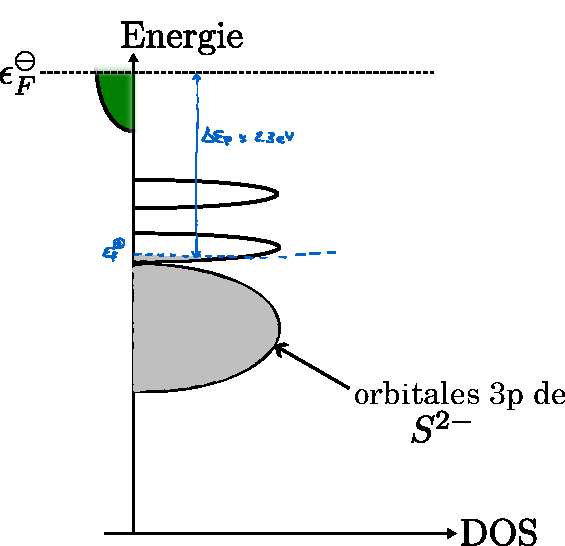
\includegraphics[height=5cm]{Ex17/Corr02b} & 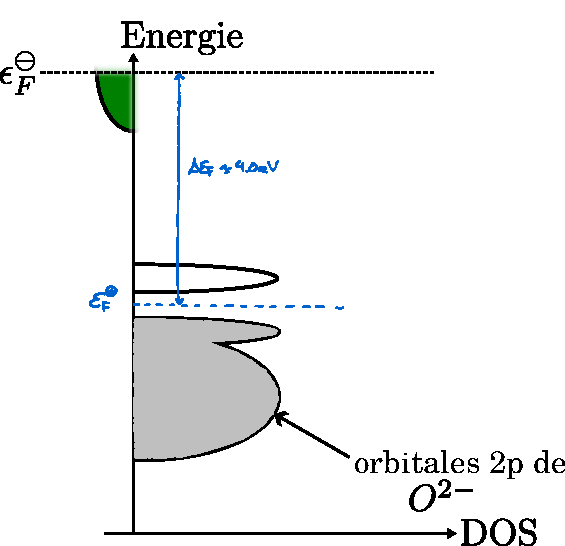
\includegraphics[height=5cm]{Ex17/Corr02c} & 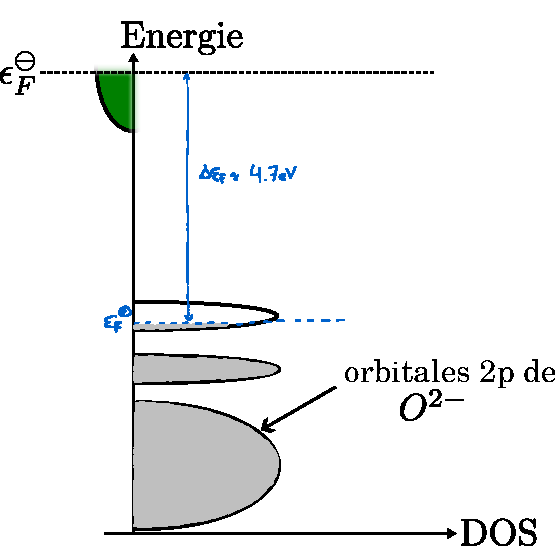
\includegraphics[height=5cm]{Ex17/Corr02d}
\end{tabular}\end{center}}

\paragraph*{Influence de la nature des éléments chimique sur la tension à courant nul}

\Q Pourquoi la tension dans les composés soufrés évolue-t-elle en général sur une plage de potentiel plus large que celle d'un oxyde équivalent ?
\solution{Dans le cas des composés soufrés, on observe que l'OCV indique que $\Delta \epsilon_F$ évolue sur la plage 2.0-2.6 \si{\electronvolt}. Du fait du caractère plus diffus des orbitales $3p$ du soufre par rapport à celles de l'oxygène $2p$, on s'attend à ce que le recouvrement entre les orbitales du métal et du soufre soit plus importante qu'entre le métal et l'oxyde (caractère covalent plus marqué). \\
Par conséquent, la densité d'état (DOS) des orbitales $d$ du titane lié au soufre sera plus élargie en énergie que celle d'un métal dans un composé oxydé (c.-à-d. lié à un oxygène).}

\Q Dans le composé \ce{LiCoO2}, on observe deux régimes remarquables d'évolution de la tension avant et après $x=0.5$. Ces deux régimes ne sont pas observés dans le composé \ce{Li_x Co PO4}. Expliquer l'origine électronique de cette différence.
\solution{Les deux régimes sont dus à la superposition de la DOS des orbitales $2p$ avec la DOS des orbitales $3d(t_{2g})$ du métal. Ainsi, lors de l'oxydation, les orbitales $t_{2g}$ les plus hautes en énergie se vident, ce qui permet un rapprochement du niveau de Fermi des niveaux $2p$ de l'oxygène. Or, dans le domaine conjoint $2p-3d(t_{2g})$, les orbitales $d$ sont hybridées avec les orbitales $p$ (=caractère covalent plus marqué).\\
Ainsi, les oxygènes subissent une oxydation partielle pour $x > 0.5$ qui s'accompagne de modifications structurales (rapprochement des plaques$\ldots$).}

\Q Commenter l'évolution de la position des orbitales $p$ lors du passage de $\ce{S^{2-}}$, $\ce{O^{2-}}$ et $\ce{PO4^{2-}}$.
\solution{Dans le phosphate, le phosphore est au degré d'oxydation +V. Il va donc exercer un effet inductif et mésomère attracteur sur l'oxygène. \\
Les orbitales $3p$ de \ce{S^{2-}} sont plus hautes en énergie que les orbitales $2p$ de \ce{O^{2-}} (nombre quantique principal plus grand). Dans le phosphate, les effets électroniques abaissent en énergie les orbitales $2p$. On a donc naturellement l'inégalité suivante en énergie :
\begin{align*}
E (3p, \ce{S^{2-}}) > E (2p, \ce{O^{2-}}) > E (2p, \ce{PO_4^{3-}})
\end{align*}}

\Q Commenter l'influence de l'anion sur la position des orbitales des métaux.
\solution{
L'énergie des orbitales $3d$ est influencée par le caractère inductif attracteur de l'anion. Plus un anion est attracteur, plus les orbitales $3d$ peuvent perdre facilement leurs électrons, plus l'énergie des orbitales $3d$ est faible :
\begin{align*}
E (3d, \ce{M-S}) > E (3d, \ce{M-O}) > E (3d, \ce{M-PO_4})
\end{align*}}

\Q En déduire pourquoi la tension à circuit-ouverte est quasiment constante pour $\ce{Li_xCoPO4}$.
\solution{
Du fait du caractère électronique attracteur du phosphore, on s'attend à ce que les orbitales moléculaires des phosphates aient recouvrement plus faible avec les orbitales $3d$ du métal que dans les oxydes. Par conséquent, les atomes métalliques sont "plus isolés". De plus, le DOS des orbitales $2p$ de l'oxygène étant énergétiquement distante de celle des orbitales $3d(e_g)$ du métal, on ne s'attend pas à avoir de transition dû à des phénomènes d'hybridation.\\
Puisque le DOS $3d(e_g)$ est très étroit, on a l'impression que le potentiel ne change presque pas.}

\paragraph*{Données}
\begin{itemize}
\item Numéro atomique $Z$ : Ti - 22, Co - 27, P - 15 ;
\item Nombre d'Avogadro : $N_A = 6.02 \cdot 10^{23} ~ \si{\per\mole}$ ;
\item Charge élémentaire de l'électron : $e = 1.6 \cdot 10^{-19} ~ \si{\coulomb}$.
\end{itemize}

